\section{Hnadwriting Generation}


\subsection{ScrabbleGAN}

I decided to implement the ScrabbleGAN \cite{ScrabbleGAN} architecture, which is able to generate handwriting text from script with various lengths and styles. The fundamental choice was either to work with online or offline data. I chose to focus on the latter. 


\begin{figure}[h]
\centering
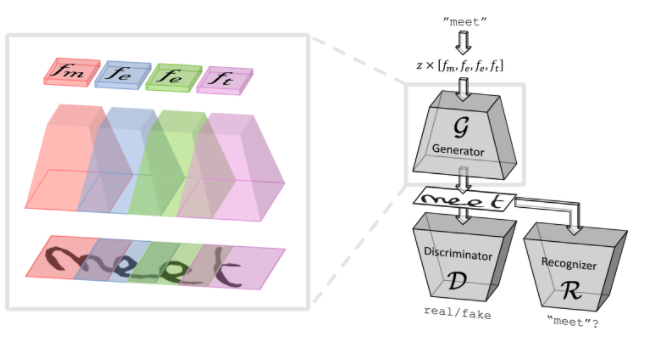
\includegraphics[scale=0.7]{scrabblegan}
\caption{ScrabbleGAN structure}
\label{fig:x cubed graph}
\end{figure}

There are a few modifications from the original GAN structure, that make this model a suitable solution to generate handwriting in different styles and lengths.


\begin{enumerate} 
 	\item Add a recognizer component - that encourage the network to generate meaningful and readable texts. 
 	\item Local embedding of each character with overlapping. The final image is generated by convolutions that allow overlapping between the characters initial embeddings, so the model learns how to generate transitions between characters. 
\end{enumerate} 

The model contains around 50 million parameters, including attention blocks, residual blocks and conditional batch normalization layers, as purposed in the original paper.


\section{Explainability}


\subsection{Extract latent space structure from a trained GAN}

An agnostic method to discover latent space linear directions is presented in the paper - 
in Unsupervised Discovery of Interpretable Directions in the GAN Latent Space paper - \cite{10}.

\subsubsection{Main idea}

The idea is to build a model on top of the generator, that will approximate meaningful directions (linear vectors). It contains two trained sub-models - A and R.
The A sub-model produces the meaningful linear directions in latent space. From these directions, we produce shifted noise vectors.  The generator generates images from the original noise vectors and from the shifted ones. The R sub-model reconstructs the directions from the two generated images.


\begin{figure}[h]
\centering
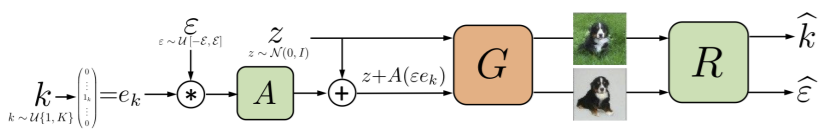
\includegraphics[scale=0.7]{unsupervised_scheme}
\caption{unsupervised discovery of latent space direction scheme as proposed in the original paper}
\label{fig:x cubed graph}
\end{figure}

\subsubsection{Algorithmic Flow}

The columns of A are the shifts in the latent space, so by choosing two variables - column $k$ and size $\epsilon$, we define a transformation from vectors in latent space to another vector in latent space, shifted by $\epsilon$ times the $k'th$ column of A.

\begin{enumerate}
\item Generate random $k, \epsilon$
\item Generate $z$, $z_{(k, \epsilon)}$	
\item Generator generate two images, $G_{z}$, $G_{z(k, \epsilon)}$ 

\item	R tries to recover $k, \epsilon $ from the 		two generated images. 
	
\end{enumerate}

A tries to find directions such that R will be able to reconstruct, based on the different characteristics of the two images. I've modified the original paper structure of R, for both MNIST GAN and ScrabbleGAN: 


\begin{figure}[!tbp]
  \centering
  \begin{minipage}[b]{0.4\textwidth}
    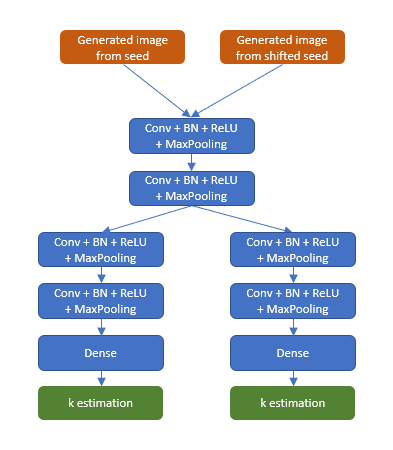
\includegraphics[width=\textwidth]{r_mnist}
    \caption{Modified R network for MNIST}
  \end{minipage}
  \hfill
  \begin{minipage}[b]{0.4\textwidth}
    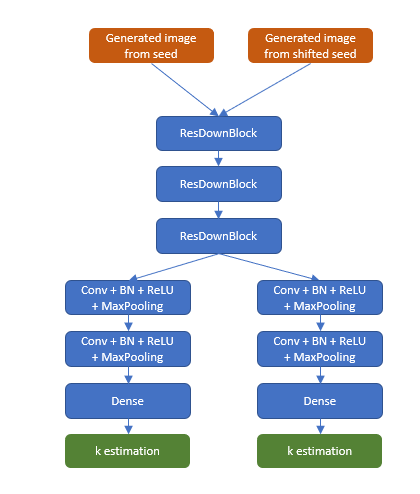
\includegraphics[width=\textwidth]{r_scrabble}
    \caption{Modified R network for SrabbleGAN}
  \end{minipage}
\end{figure}



\subsection{Attention Mechanism}


\subsubsection{In GAN models}

In GAN models, it was introduced in SAGAN paper \cite{SAGAN} the implementation of this idea as layers of the discriminator and generator:


\begin{figure}[h]
\centering
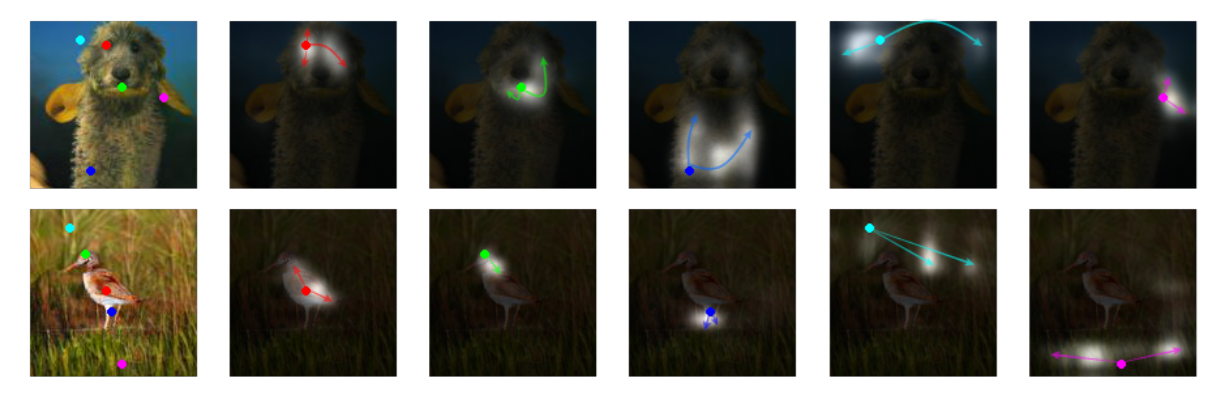
\includegraphics[scale=0.5]{attention_SAGAN}
\caption{Self Attention maps as presented in SAGAN paper}
\label{fig:x cubed graph}
\end{figure}


Self-Attention Generative Adversarial Networks is the implementation of attention mechanism in GAN architecture.

\subsubsection{Algorithmic Flow}

 
The implementation is pretty straight forward from the the plot at Fig 5.6.


All three parts - K, Q and V are derived by separate convolutions of the inputs. 

The keys and queries create (by matrix multiplication and soft-max activation) the attention maps. For each generated output of the model, there is a correlated attention map at the size of the layer input. It is activated where the model should put attention to, and zeros areas that are needed to be ignored.

This map is multiplied by the Values and creates a generated output. 
Each part of the output (pixels in our case) has access to information from all across the input thanks to the attention mechanism. This is why it sometimes called Non Local Blocks. With traditional architectures, each pixel won't have this various access to all parts of the input, but only to the local features in its area.


\begin{figure}[h]
\centering
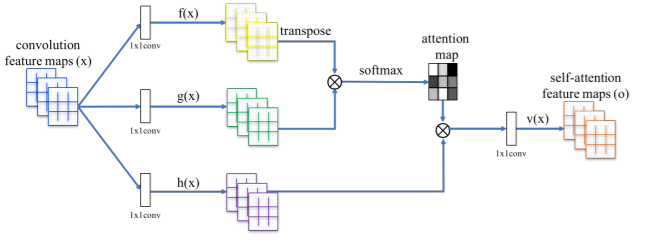
\includegraphics[scale=0.5]{attention_layer_sagan}
\caption{Self Attention layer as proposed in SAGAN paper}
\label{fig:x cubed graph}
\end{figure}



\subsection{InfoGAN}

InfoGAN is an extension of GAN, that by modifying both the latent space and the objective goal is able to learn distangled representations.  

\subsubsection{Main idea}


InfoGAN adds a categorical feature c and countinous features $c_{i}$ to the latent space. It tries to recover only them and not the whole latent space. One can think of this framework as a relaxed version of the BiGAN - we are enforcing some restrictions on the generator, forcing him to preserve the latent space structure. 



\begin{figure}[h]
\centering
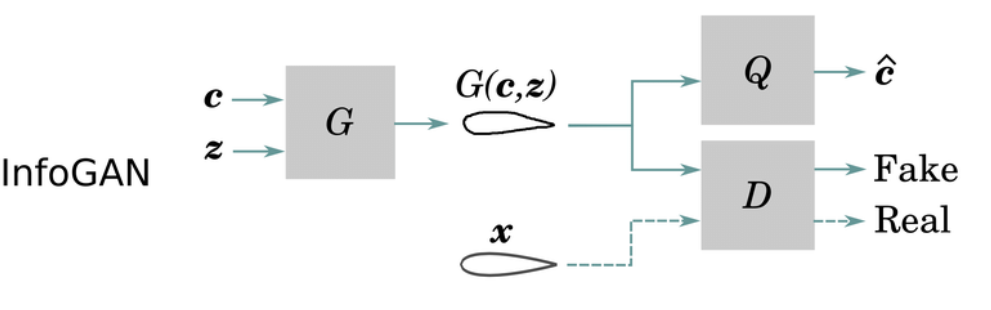
\includegraphics[scale=0.5]{InfoGAN}
\caption{InfoGAN structure \cite{14}}
\label{fig:x cubed graph}
\end{figure}



\subsubsection{Implementation details}


We draw the codes from a known distribution, and the encoder Q tries to recover the distribution they were drawn from. 

the new loss term is:

$\underset{G}{min}\underset{D}{max}V(D,G)- \lambda I(c,G(z,c))$
where V(G, D) is the vanilla GAN loss term, and I is the information between the codes and the image generated using them as part of the seed. 

The loss term is calculated by a probability function:

\centerline{$L_{I}(c, c_{i}, \varphi_{c}, \varphi_{c_{i}}) = -log(P(c|U_{\varphi_{c}})) -log(P(c_i|N_{\varphi_{c_i}}))$}

$\varphi_{c}$ are the parameters to fix a discrete distribution (softmax activations), and $\varphi_{c_{i}}$ are the parameters to fix a normal distribution (mean and variance), and these are the Q network outputs.
We measure I by Q network, that predicts the distribution of these additional variable.
 

